\section{Numerical and Experimental Evaluation} \label{sec:experiments}

The goal of this section is to evaluate the proposed control framework and the adaptation to the original SC method. To this end, we define the following metrics:
\begin{itemize}
    \item \textit{average stage cost}: this performance metric is computed by averaging the stage cost evaluated at each time step. Task duration and cost scheduling is kept fixed among all the experiments.  
    \item \textit{cumulative constraints violation}: as each barrier function is, by definition, negative outside of the safe set, we define the following metric as a proxy for the size of the constraint violation along the duration of an experiment:
    \begin{equation*}
        \Delta^{i}_{tot} = \sum\limits_{t=0}^{T_{exp}} \max(0, -h^i(\vect{x}_t)),
    \end{equation*}
    referring to the $i$th ZBF.
    \item \textit{average interaction wrench}: average wrench which is exerted on the environment during the execution of the task
    \item \textit{dissipated power}: during an ideal interaction with an articulated object, power is minimally dissipated. Therefore, we use the dissipated power as an efficiency metric:
    \begin{equation}
        P_{diss} = \sum\limits_{0}^{T_{exp}} -\command^T \boldsymbol{\tau}_{ext}.
    \end{equation}
\end{itemize}
The simulation experiments are conducted on a dynamic manipulator model as described by \eqref{eq:eom}. To this end, we use the Raisim physics engine \cite{raisim}. The manipulation tasks consist of maneuvering different articulated objects: a \textit{shelf}, a \textit{dishwasher}, a \textit{microwave} and a \textit{drawer} as shown in \fig\ref{fig:object_manipulation}. They differ in type and orientation of the joint. The \textit{shelf} and \textit{microwave} have a vertical revolute joint, the \textit{dishwasher} has a horizontal revolute joint, while the \textit{drawer} has a horizontal prismatic joint. The simulated manipulator is controlled using a PI low-level velocity controller running at 1KHz. Imperfect velocity control is modeled by compensating only 90\% of the gravity terms.
  
\begin{figure}[t]
\centering
  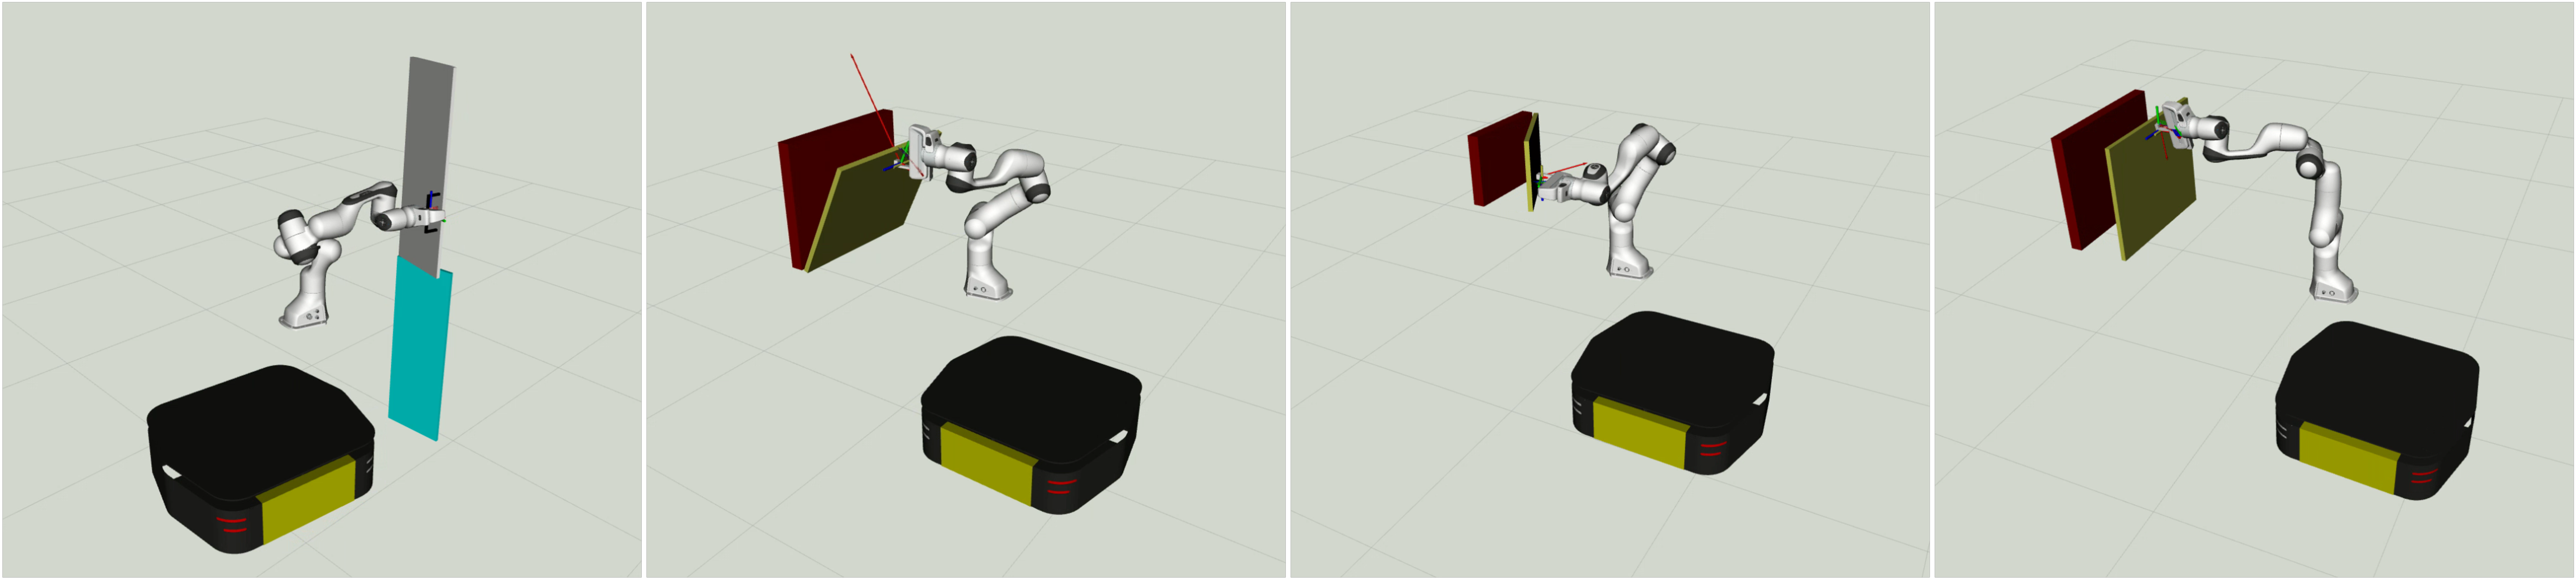
\includegraphics[width=\columnwidth]{framework_manipulation/figures/mosaics/articulated_objects_sim.pdf}
  \caption{The four articulated objects used in our simulation evaluations. From left to right: shelf, dishwasher, microwave, drawer.} \label{fig:object_manipulation}
\end{figure}

%\subsection{Power consumption}
%In this experiment we look at the effect of the power term in the task execution. As we can see in \fig \ref{fig:power_cost_comparison}, the power cost is effective in decreasing the energy dissipation during the manipulation task. For each of the experiments where the power cost is active we set $w_p=10$ and $p_{max} = 0.0$. For all experiments we use $50$ samples as they are a good trade-off between control-frequency and performance. We observe that in all experiments the robot is able to accomplish the task (fully open the articulated object). 

%\begin{figure}[t]
%\centering
%  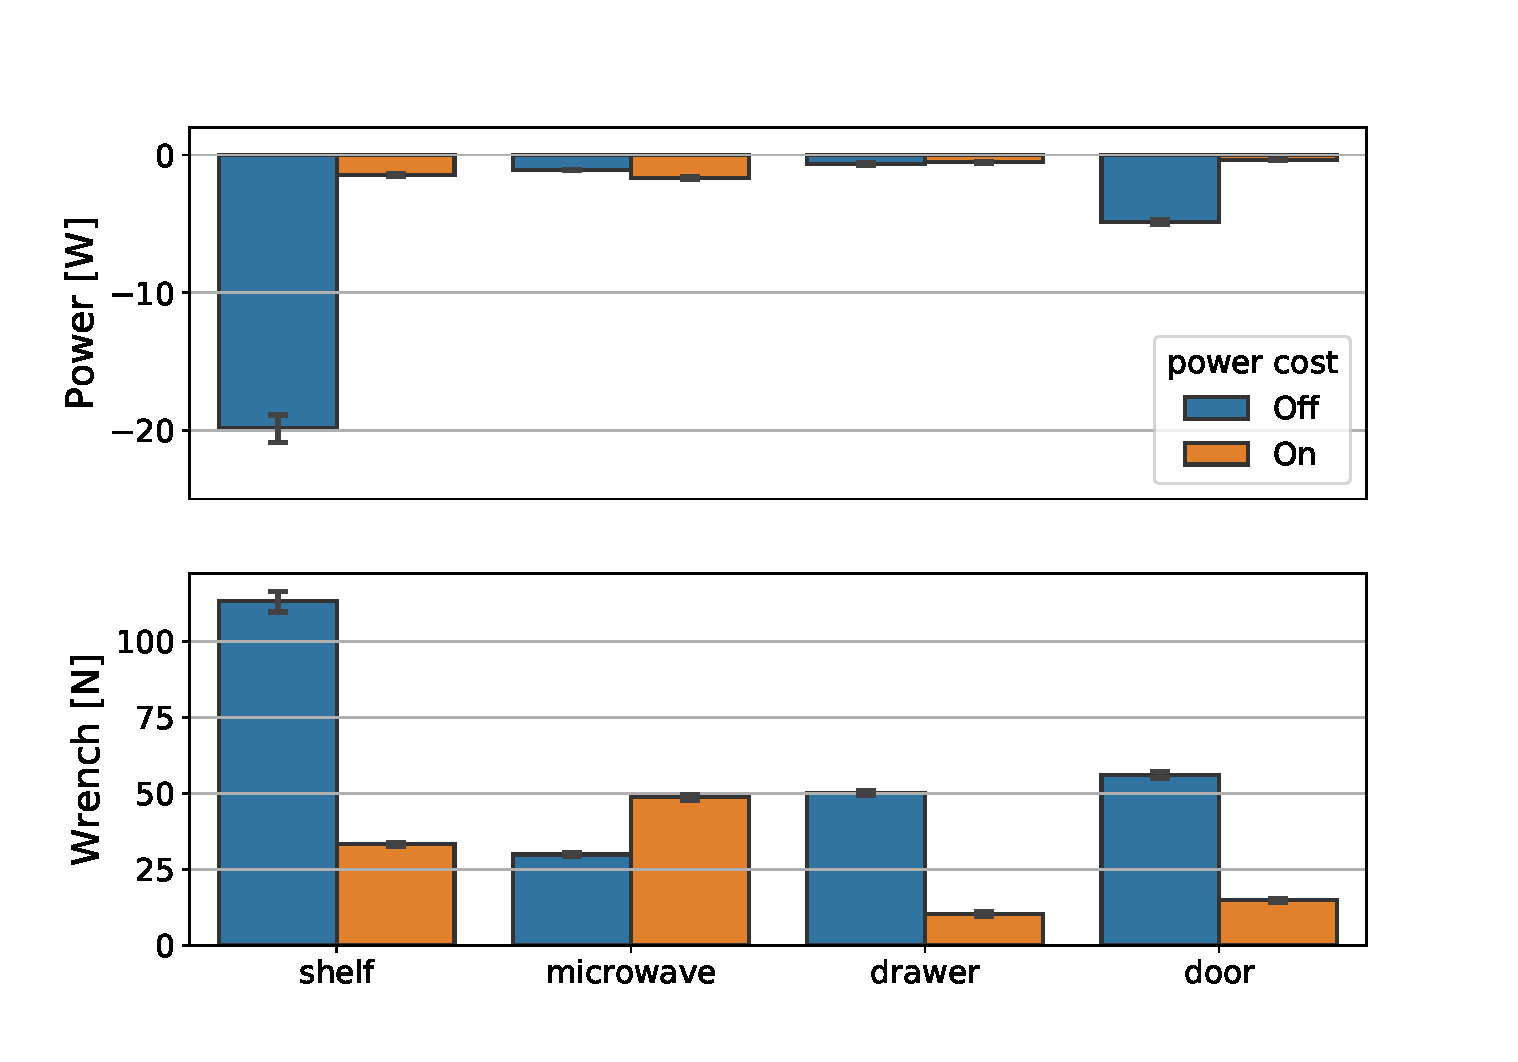
\includegraphics[width=\columnwidth]{figures/methods_comparison/power_cost.pdf}
%  \caption{Power dissipated and wrench norm for each of the manipulated objects.} \label{fig:power_cost_comparison}
%\end{figure}


\subsection{Comparison of methods}
We briefly recap each of the control methods that are evaluated in this section. We denote each controller with $\Pi_{*}$ where $*$ can be $N,\ O,\ I,\ IO$:
\begin{itemize}
    \item[$\Pi_{N}$:] relies exclusively on a stochastic controller to generate velocity commands, namely the input is not filtered either by a FILTER-QP or a Sequential FILTER-QP
    \item[$\Pi_{O}$:] a FILTER-QP is used to optimize the input sequence received by the stochastic controller. The FILTER-QP is solved at the same rate as the low-level controller,
    \item[$\Pi_{I}$:] the Sequential FILTER-QP is used in the stochastic controller to enforce safety and passivity constraints  as described in \algo \ref{algo:sequential_qp}. No FILTER-QP is solved at higher rate in the low level controller.
    \item[$\Pi_{IO}$:] the full cascaded architecture (see \fig \ref{fig:cascaded_architecture}) is deployed, combining the previous two methods.
\end{itemize}

We evaluate the control methods in a set of experimental scenario:
\begin{enumerate}
    \item \textit{object manipulation}: we validate the applicability of the method on the challenging task of moving each of the presented 4 articulated objects,   
    \item \textit{target reaching and obstacle avoidance}: we further investigate the validity of the constraints formulation for a target reaching task in a confined environment while a sudden obstacle is placed in the workspace,
    \item \textit{robust interaction}: finally we show that the method enables robust interaction when an unforeseen event happens, in this case, the articulated object is fixed rigidly and is not able to move for a short period of time,
    \item \textit{real world experiments}: we further object manipulation and robust interaction on the real platform. 
\end{enumerate}

\vspace{0.5cm}
\subsubsection{Object manipulation}
We would like to investigate the performance of the algorithms when working close or outside the safety boundaries. To this end, in all the simulated experiments the robot starts in a configuration that is near the arm's joints limits and self-collision. The base of the robot is at $(-3.0, -3.0)$, outside of the prescribed position limits of $[(2.0, 2.0), (-2.0, -2.0)]$. The robot is endowed with the task to open an articulated object moving from its starting location. We perform 10 runs for each articulated object and for each control method.

The results of the experiments are summarized in \fig \ref{fig:methods_comparison}. In all cases, filtering the velocity commands has a beneficial effect. We observer a reduction of cumulative joint limits as well as self collision limits violation. We deduce that filtering the input sequence has a beneficial effect. The improvement is even more pronounced when the filtering is tightly coupled to the sampling based controller through the Safety FILTER-QP. $\Pi_{I}$ and $\Pi_{IO}$ have the best performance suggesting that in a low sampling regime, the optimization problem helps to adapt the input sequence to reduce quickly the amount of constraints violation. In \fig \ref{fig:self_collision_violation} the naive controller $\Pi_{N}$ even experiences a dramatic failure which is not visible because of plots limits. This is instead never for the other methods. 

The dissipated power is similar across the methods even though a positive trend is observed when using the adaptations proposed in this paper. A qualitative analysis has shown that the simulation wrench measured during a simulated rollout can be inaccurate. In fact, the algorithm uses big time steps to trade-off simulation accuracy with speed. An accurate evaluation of the simulator fidelity, especially when dealing with dynamic effects is a complex task that we leave to future works. In this work instead, we activate the passivity enforcing constraint only in the outer FILTER-QP has this works on real wrench measurements at high rates. Furthermore passivity is mainly a mechanism designed to reach to unforeseen events. As these are not, by definition modeled, the simulated rollouts do not predict the true evolution of the interaction wrench and therefore passivity might be enforced in a counterproductive way.

Overall, the simulated experiments confirm the validity of the full framework implemented in $\Pi_{IO}$ but the performance differences are not striking. We think that this is due to the low change of hitting the constraints, especially when the sampling based controller is aware of dangerous configuration through a well-engineered cost function. In fact, high cost on safety critical objectives has the effect of "trimming" bad trajectories leaving little to do in the post-processing stage performed by the FILTER-QP and Sequential FILTER-QP. For this reason, in the following we present a second simulation experiment which constitute a challenge for a purely sampling based controller. 

\begin{figure}[t]
\centering
\hspace*{-0.2cm}
\vspace*{0.15cm}
\begin{subfigure}{1\columnwidth}
    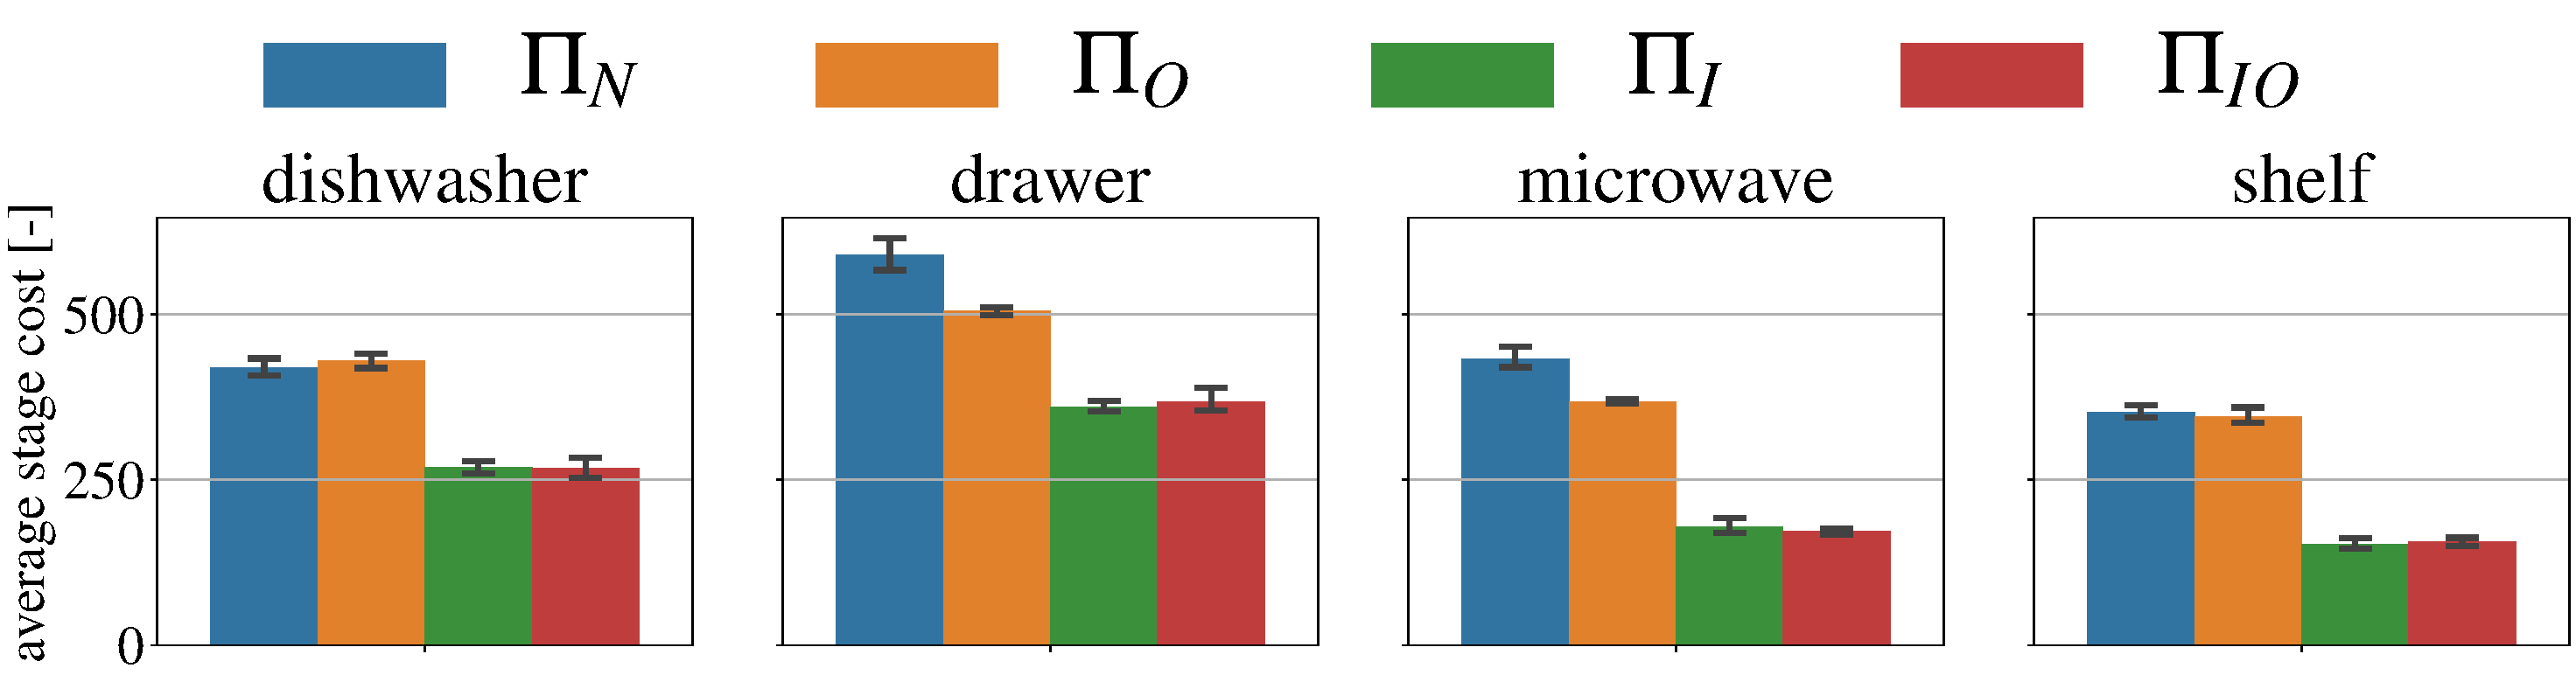
\includegraphics[width=\linewidth]{figures/methods_comparison/average_stage_cost.pdf}
\end{subfigure}%
\hfill
\hspace*{-0.2cm}
\vspace*{0.1cm}
\begin{subfigure}{\columnwidth}
    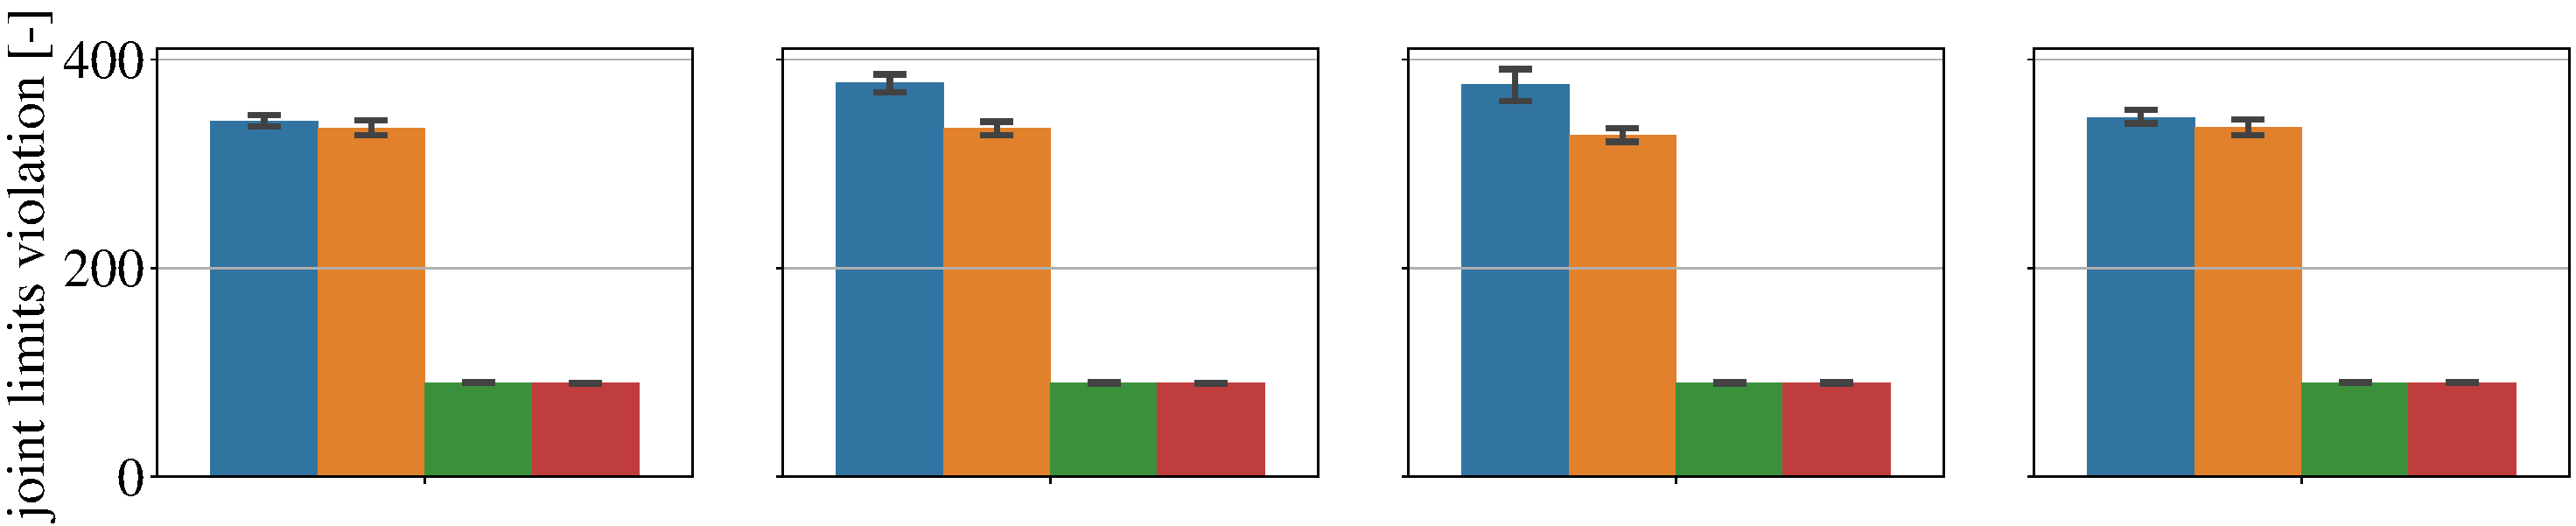
\includegraphics[width=\linewidth]{figures/methods_comparison/joint_limits.pdf}
\end{subfigure}%
\hfill
\hspace*{-0.2cm}
\vspace*{0.1cm}
\begin{subfigure}{\columnwidth}
    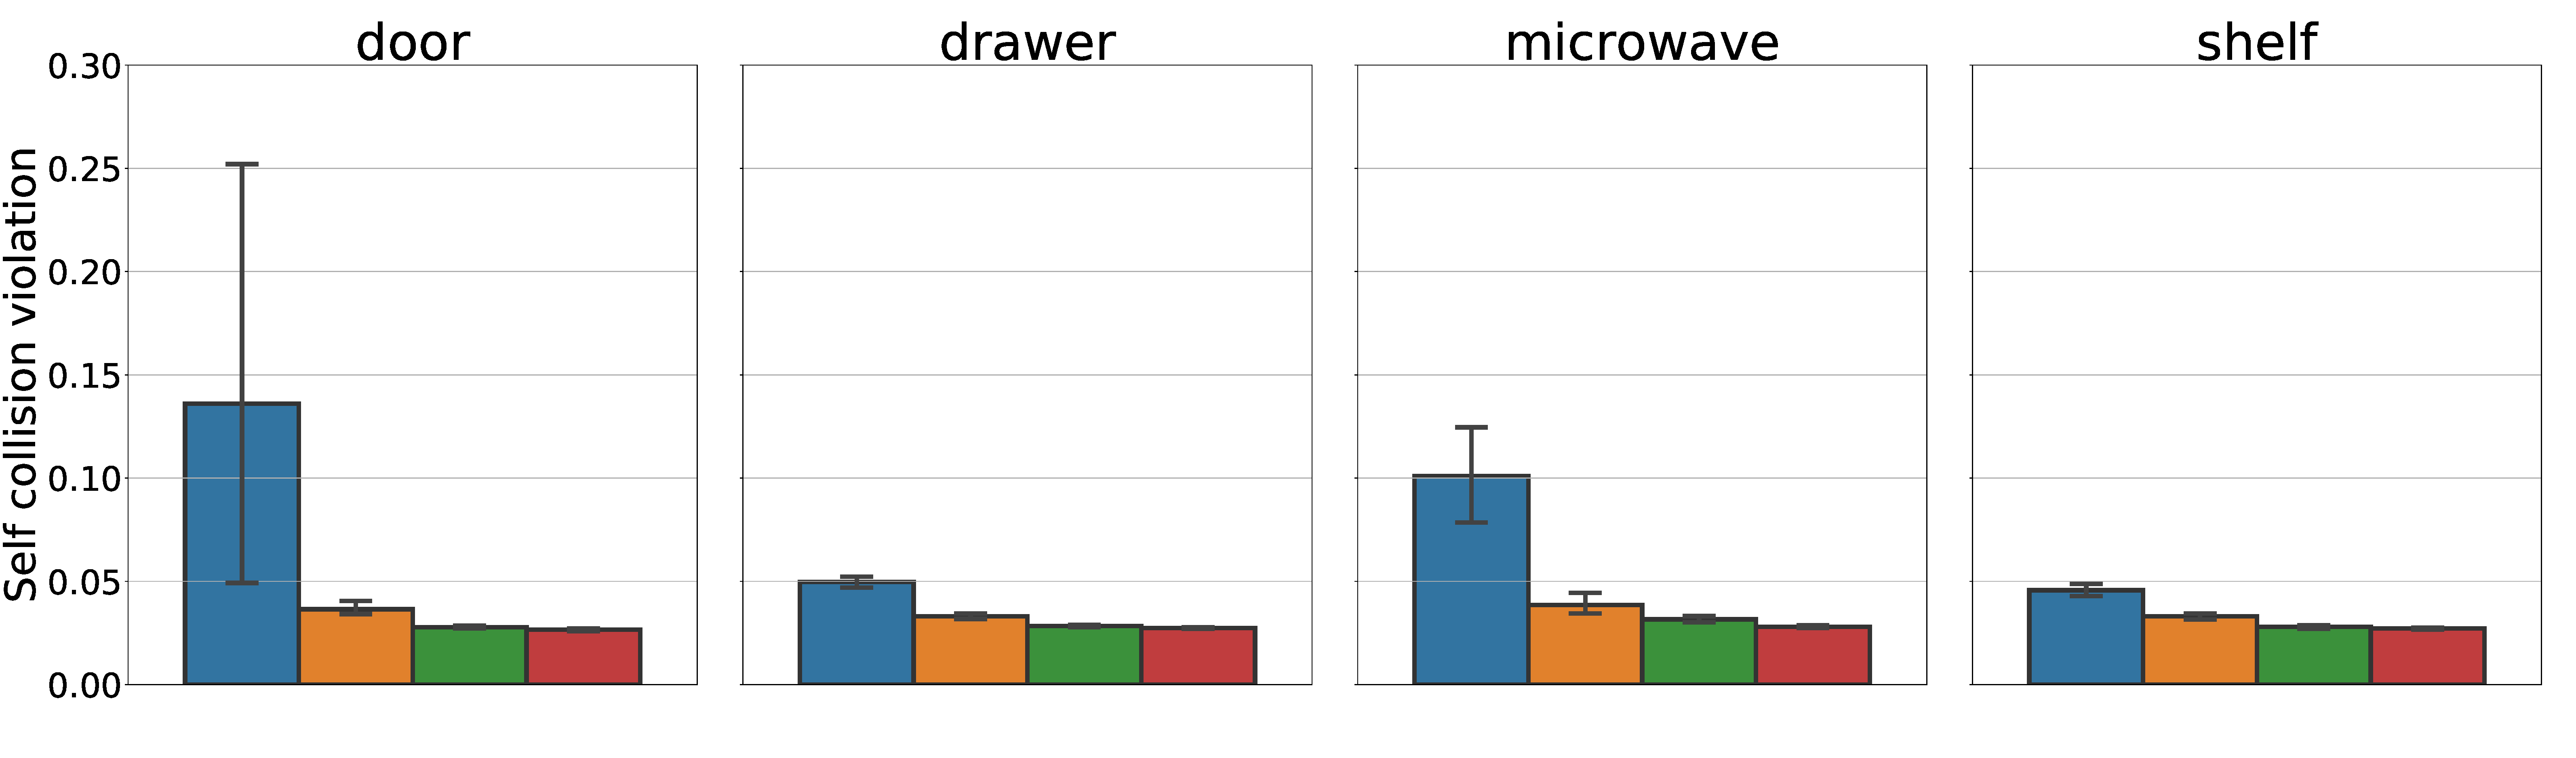
\includegraphics[width=\linewidth]{figures/methods_comparison/self_collision.pdf}
\end{subfigure} \label{fig:self_collision_violation}
\hspace*{-0.2cm} 
\vspace*{0.1cm}
\begin{subfigure}{\columnwidth}
    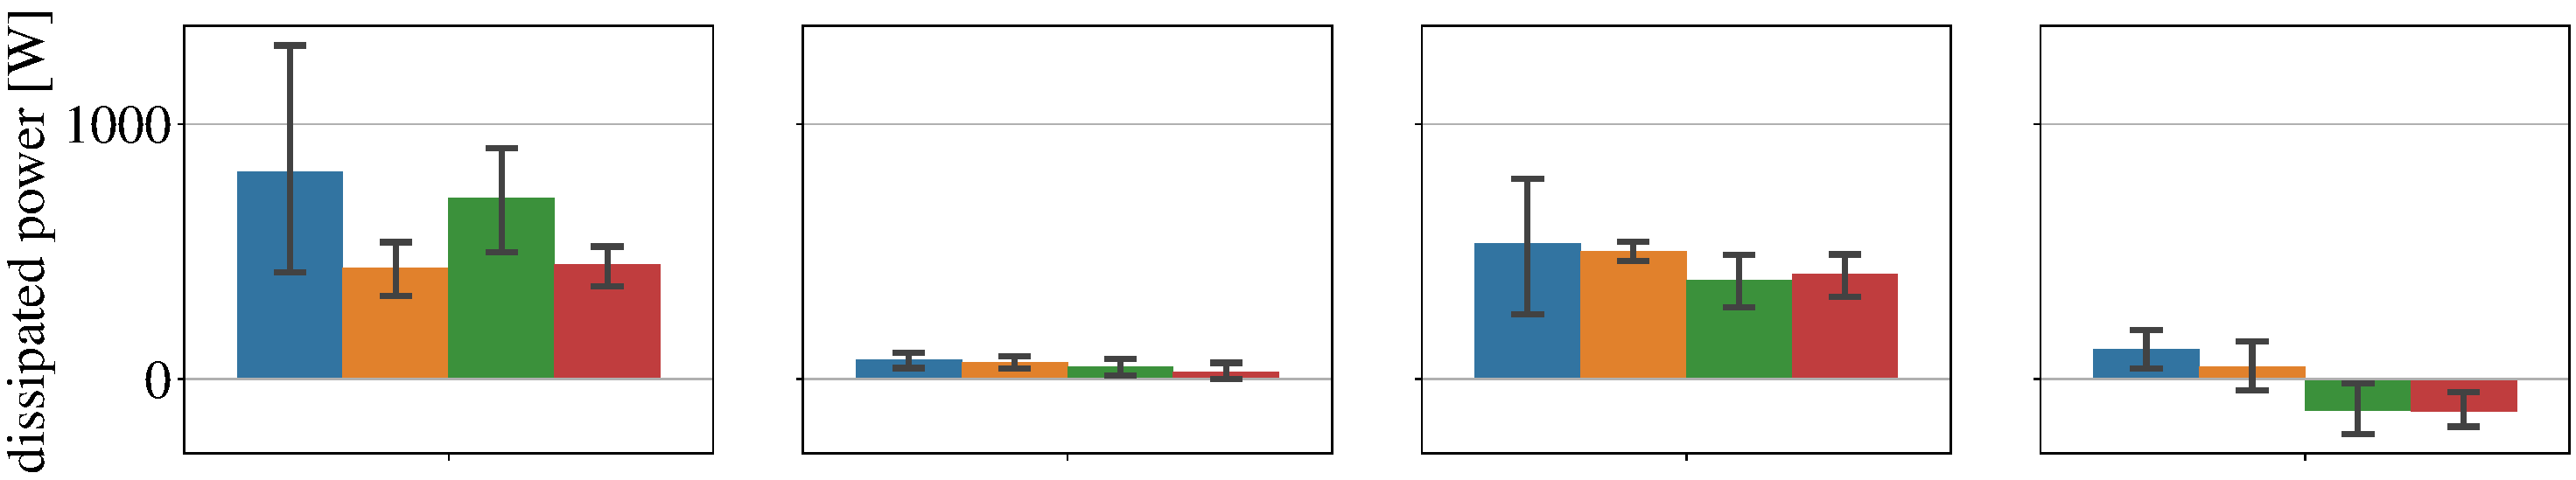
\includegraphics[width=\linewidth]{figures/methods_comparison/dissipated_power.pdf}
\end{subfigure}
\hfill
\caption{Comparison between the different control methods when the FILTER-QP is used in different stages of the cascaded architecture. Results are separate by manipulation task. The self-collision metric accounts also for the arm-reach constraint as they share the same implementation. \add{Where the bar goes high there is an outlier at 3.4}}\label{fig:methods_comparison}
\end{figure}

\vspace{0.5cm}
\subsubsection{Target reaching and obstacle avoidance}
The naive stochastic controller relies on a task-encoding cost formulation and sampling to generate "good" rollouts. This method faces two main challenges:
\begin{itemize}
    \item the cost needs to be nicely tuned in order to prevent edge cases where performance in chosen in lieu of safety
    \item sudden changes in the cost function lead to a drastic change in the policy distribution 
\end{itemize}
While the first issue can be addressed tuning the cost with a trial and error method, the second is more subtle. In fact, the policy should be able to quickly adapt but this can be hard to achieve sampling around the previous (outdated) input distribution. In this experiment we reproduce the described issue during a target reaching task. We place a collision sphere at each robot link and an obstacle in the robot workspace. The base motion is also constrained such that, in order to achieve the goal, the robot is forced to avoid the obstacle. The obstacle is perceived only when the robot is very close to it ($<$ 1cm). We show the end effector optimal trajectory for $\Pi_{N}$ and $\Pi_{IO}$ after the obstacle has been detected in \fig \ref{fig:rollouts_comparison}. We can see that the naive controller $\Pi_{N}$ is not able to quickly adapt to the unforeseen cost change and instead is trapped in a high cost region where it is hard to find a good trade-off between obstacle avoidance and the target reaching objective. The controller $\Pi_{IO}$ instead, immediately adapts the input sequence to comply to constraints and sampling can be later performed in a more favorable region of the input space.   

\begin{figure}[t]
\centering
\begin{subfigure}{0.48\columnwidth}
    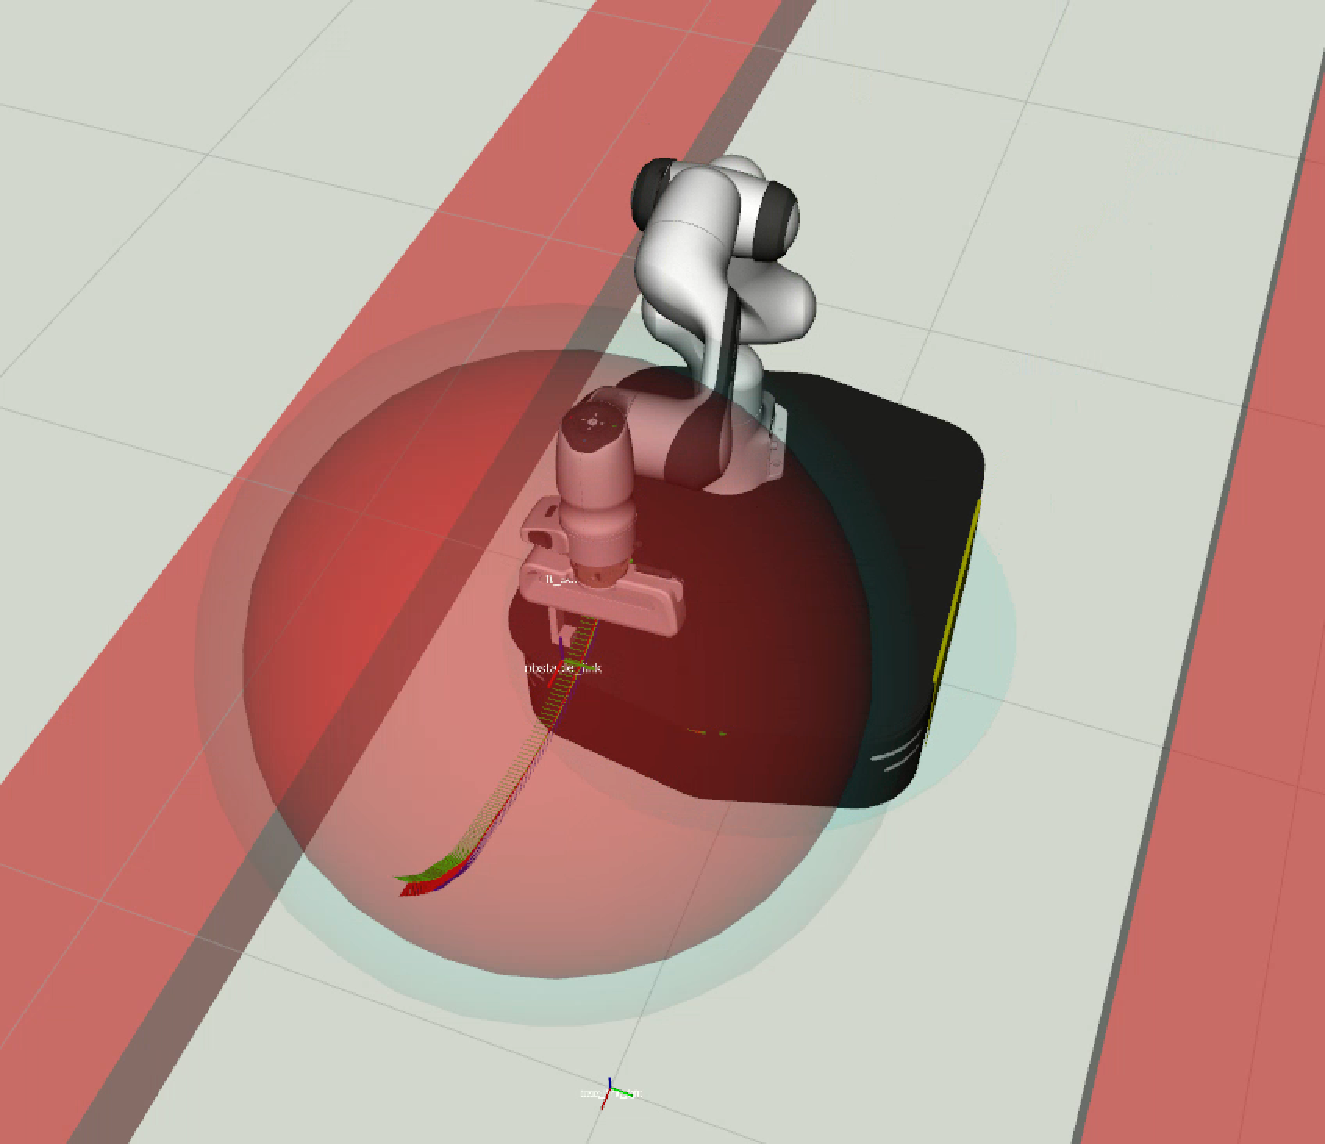
\includegraphics[width=\linewidth]{figures/obstacle_avoidance/rollouts_no_filter.pdf}
    \caption{Example rollouts of $\Pi_{N}$}
\end{subfigure}%
\hfill
\begin{subfigure}{0.48\columnwidth}
    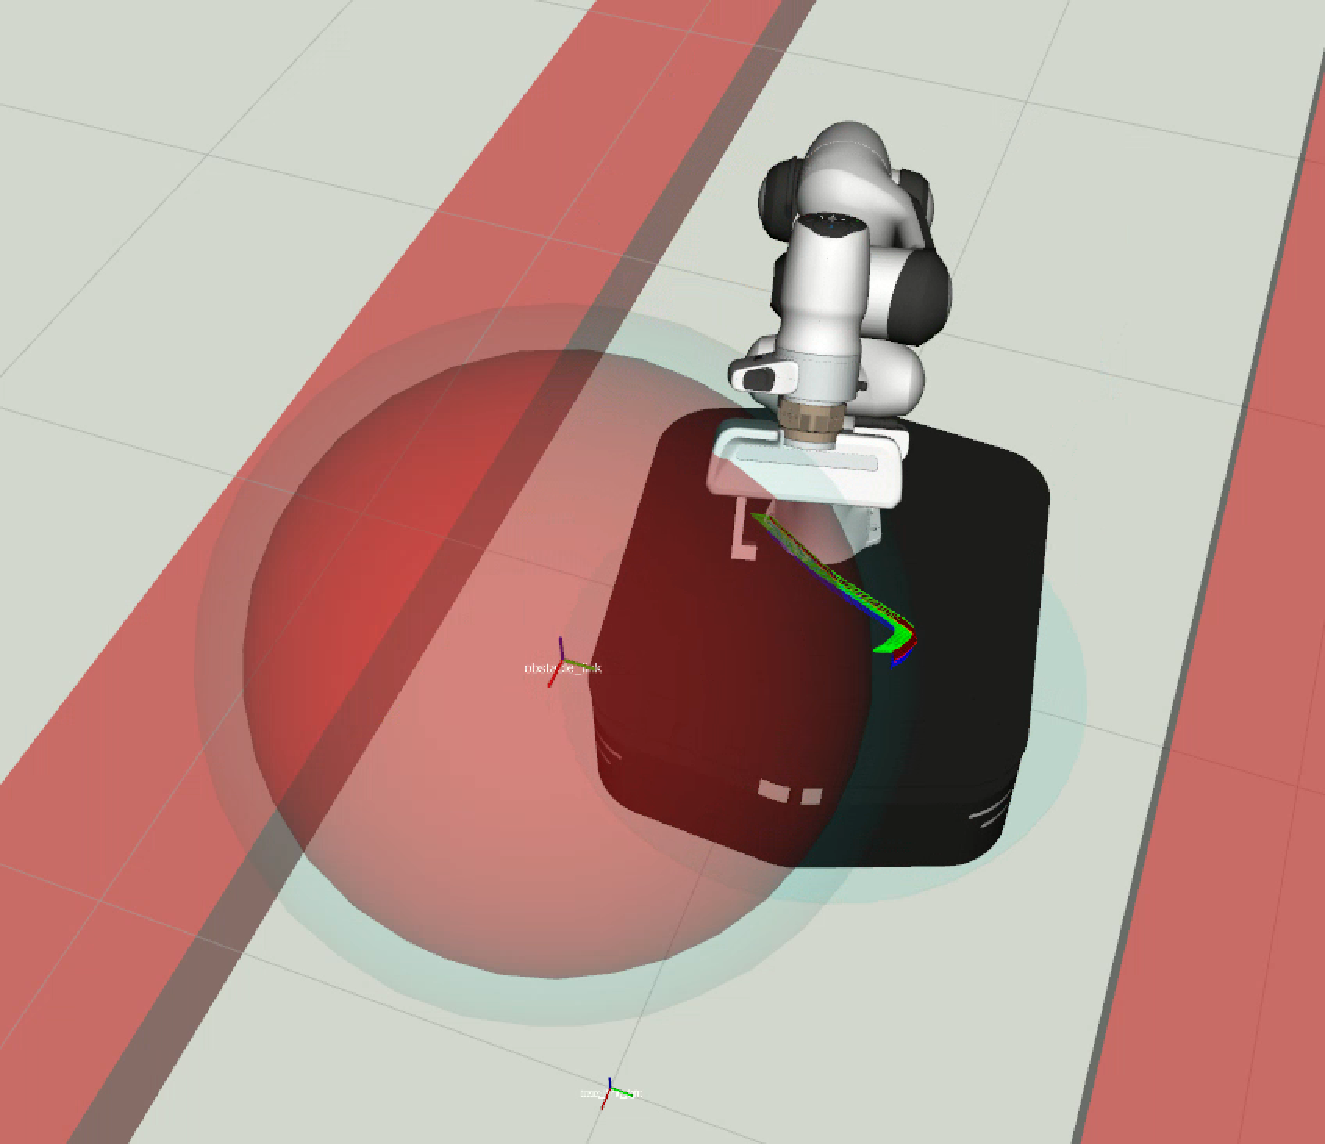
\includegraphics[width=\linewidth]{figures/obstacle_avoidance/rollouts_filter.pdf}
    \caption{Example rollouts of $\Pi_{IO}$}
\end{subfigure}%
\hfill
\caption{In the figure we visualize the optimized end effector trajectory by rolling out the optimized command. The naive controller $\Pi_{N}$ is trapped in a high region cost while $\Pi_{IO}$ immediately react to the sudden cost change.}\label{fig:rollouts_comparison}
\end{figure}

We repeat the simulation for ten runs for each of the method. The results are summarized in \fig \ref{fig:obstacle_avoidance}. As expected, $\Pi_{IO}$ attains the best performance. We further observe that the presence of a FILTER-QP in the outer high rate loop additionally improves robustness as it enforces constraints during the open-loop execution of the optimized trajectory received by the stochastic controller. 
\begin{figure}[t]
    \centering
    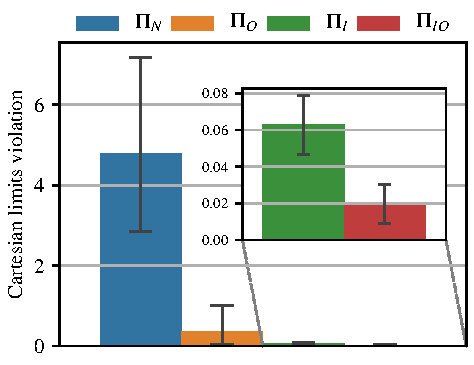
\includegraphics[width=0.7\columnwidth]{figures/obstacle_avoidance/obstacle_avoidance_test.pdf}
    \caption{Caption}
    \label{fig:obstacle_avoidance}
\end{figure}

\vspace{0.5cm}
\subsubsection{Robust interaction}
The previous validation show how the framework is powerful in addressing manipulation tasks and overcome some limitations of a naive stochastic controller. We aim to show evidence that the additional passivity enforcing constraints add robustness to the method during interaction. By adding the energy tank constraint to the optimization problem we hope to limit the maximum dissipated energy and thus generate a stable and robust interaction behavior. In this scenario, the motion of the articulated object is limited while the robot is interacting with it. We fix the object position for $5s$. After this time the object is released and is free to move within its original limits. From the results in \fig\ref{fig:tank_comparison}, we note that when the FILTER-QP is turned off and therefore no passivity is ensured, the negative power flow is not bounded, leading to high interaction wrenches. On the other hand, when the energy tank is used, only a maximal amount of energy, namely that stored in the tank, can be used, regulating the overall interaction wrench.

\begin{figure}[t]
\centering
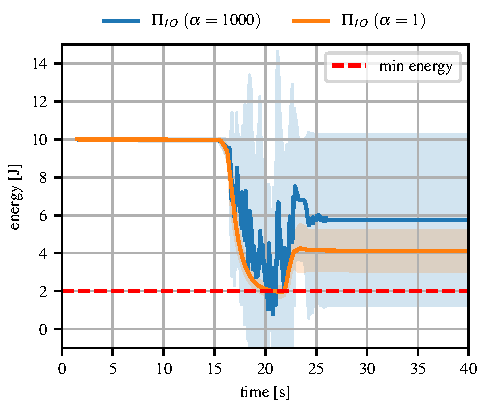
\includegraphics[width=0.8\columnwidth]{figures/fix_experiment/passivity_coefficient_comparison.pdf}
\caption{In this figure we show the chattering effect happening when the constraints is enforced with $\alpha = 1/dt = 1000$. Instead a lower $\alpha$ greatly alleviates this effect.  }\label{fig:tank_as_zbf}
\end{figure}

\begin{figure}[t]
\centering
\hspace*{-0.0cm} 
\begin{subfigure}{0.8\columnwidth}
    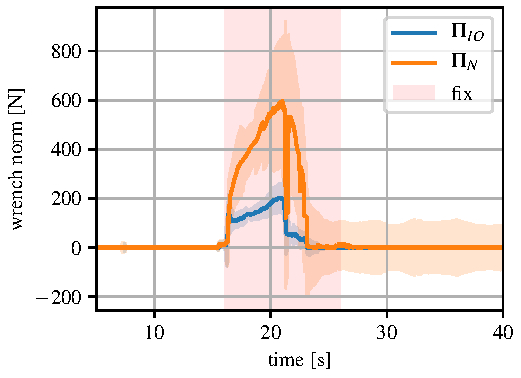
\includegraphics[width=\linewidth]{figures/fix_experiment/wrench_with_without_tank.pdf}
    \caption{The red shaded area shows the time interval when the object is fixed. Note that this might vary for each experiment as the object reaches the prescribed position at different time points.}
\end{subfigure}
\hspace*{-0.0cm} 
\begin{subfigure}{0.8\columnwidth}
    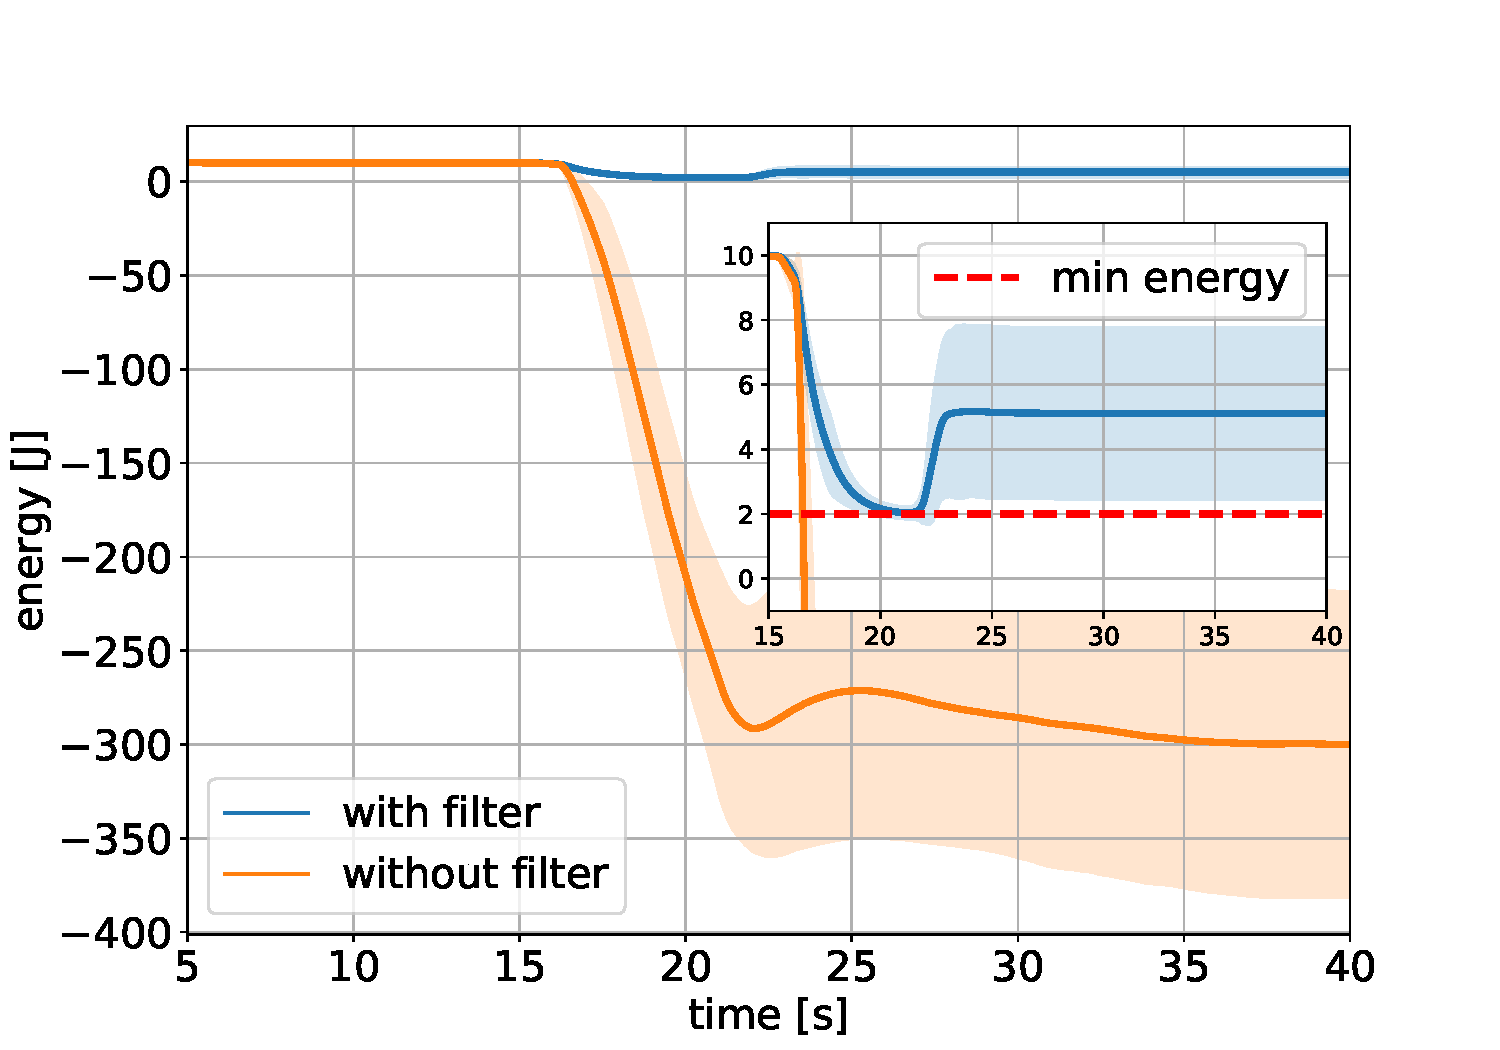
\includegraphics[width=\linewidth]{figures/fix_experiment/energy_with_without_tank.pdf}
    \caption{While the energy is always below zero when using the filter, it drastically drops in the other case. The plotted energy is computed integrated the dissipated power during interaction.}
\end{subfigure}
\hfill
\caption{The figure shows the exerted wrench and the tank energy during the task. The filter regulates the dissipated power when energy is low in the tank, resulting in a reduced wrench when the object is "stuck". Statistics are extracted from 20 simulation runs of interaction with the \textit{shelf} object}\label{fig:tank_comparison}
\end{figure}

\vspace{0.5cm}
\subsubsection{Real world experiments}
We finaly test the developed algorithms on Our RoyalPanda test platform. It consists of a holonomic mobile base equipped with a 7-DOF manipulator. The robot's wrist mounts a 6 axis force-torque sensor and a custom set of fingers as shown in \fig\ref{fig:custom_fingers}. This hardware adaptation simplifies the problem without limiting the capabilities of the platform. We run the presented algorithm on a Intel Core i7-8550U quad-core processor (1.8 GHz, up to 4.0 GHz) and use 8 threads for parallel forward sampling of rollouts. All control parameters are summarized in \tab \add{add table of parameters}. The target velocity commands are tracked by a PI controller which converts these into motor torques. The omnidirectional base is controlled by sending velocity commands to the mecanum wheel controller. The arm's low-level controller runs at 1KHz while the base mecanum controller runs at 50Hz. The FILTER-QP and Sequential FILTER-QP are solved efficiently using the \texttt{osqp} C++ library \cite{osqp}. We measure an average solving time of $\approx 0.1$ ms.  

\begin{figure}[t]
\centering
\hspace*{-0.0cm} 
\begin{subfigure}{0.9\columnwidth}
    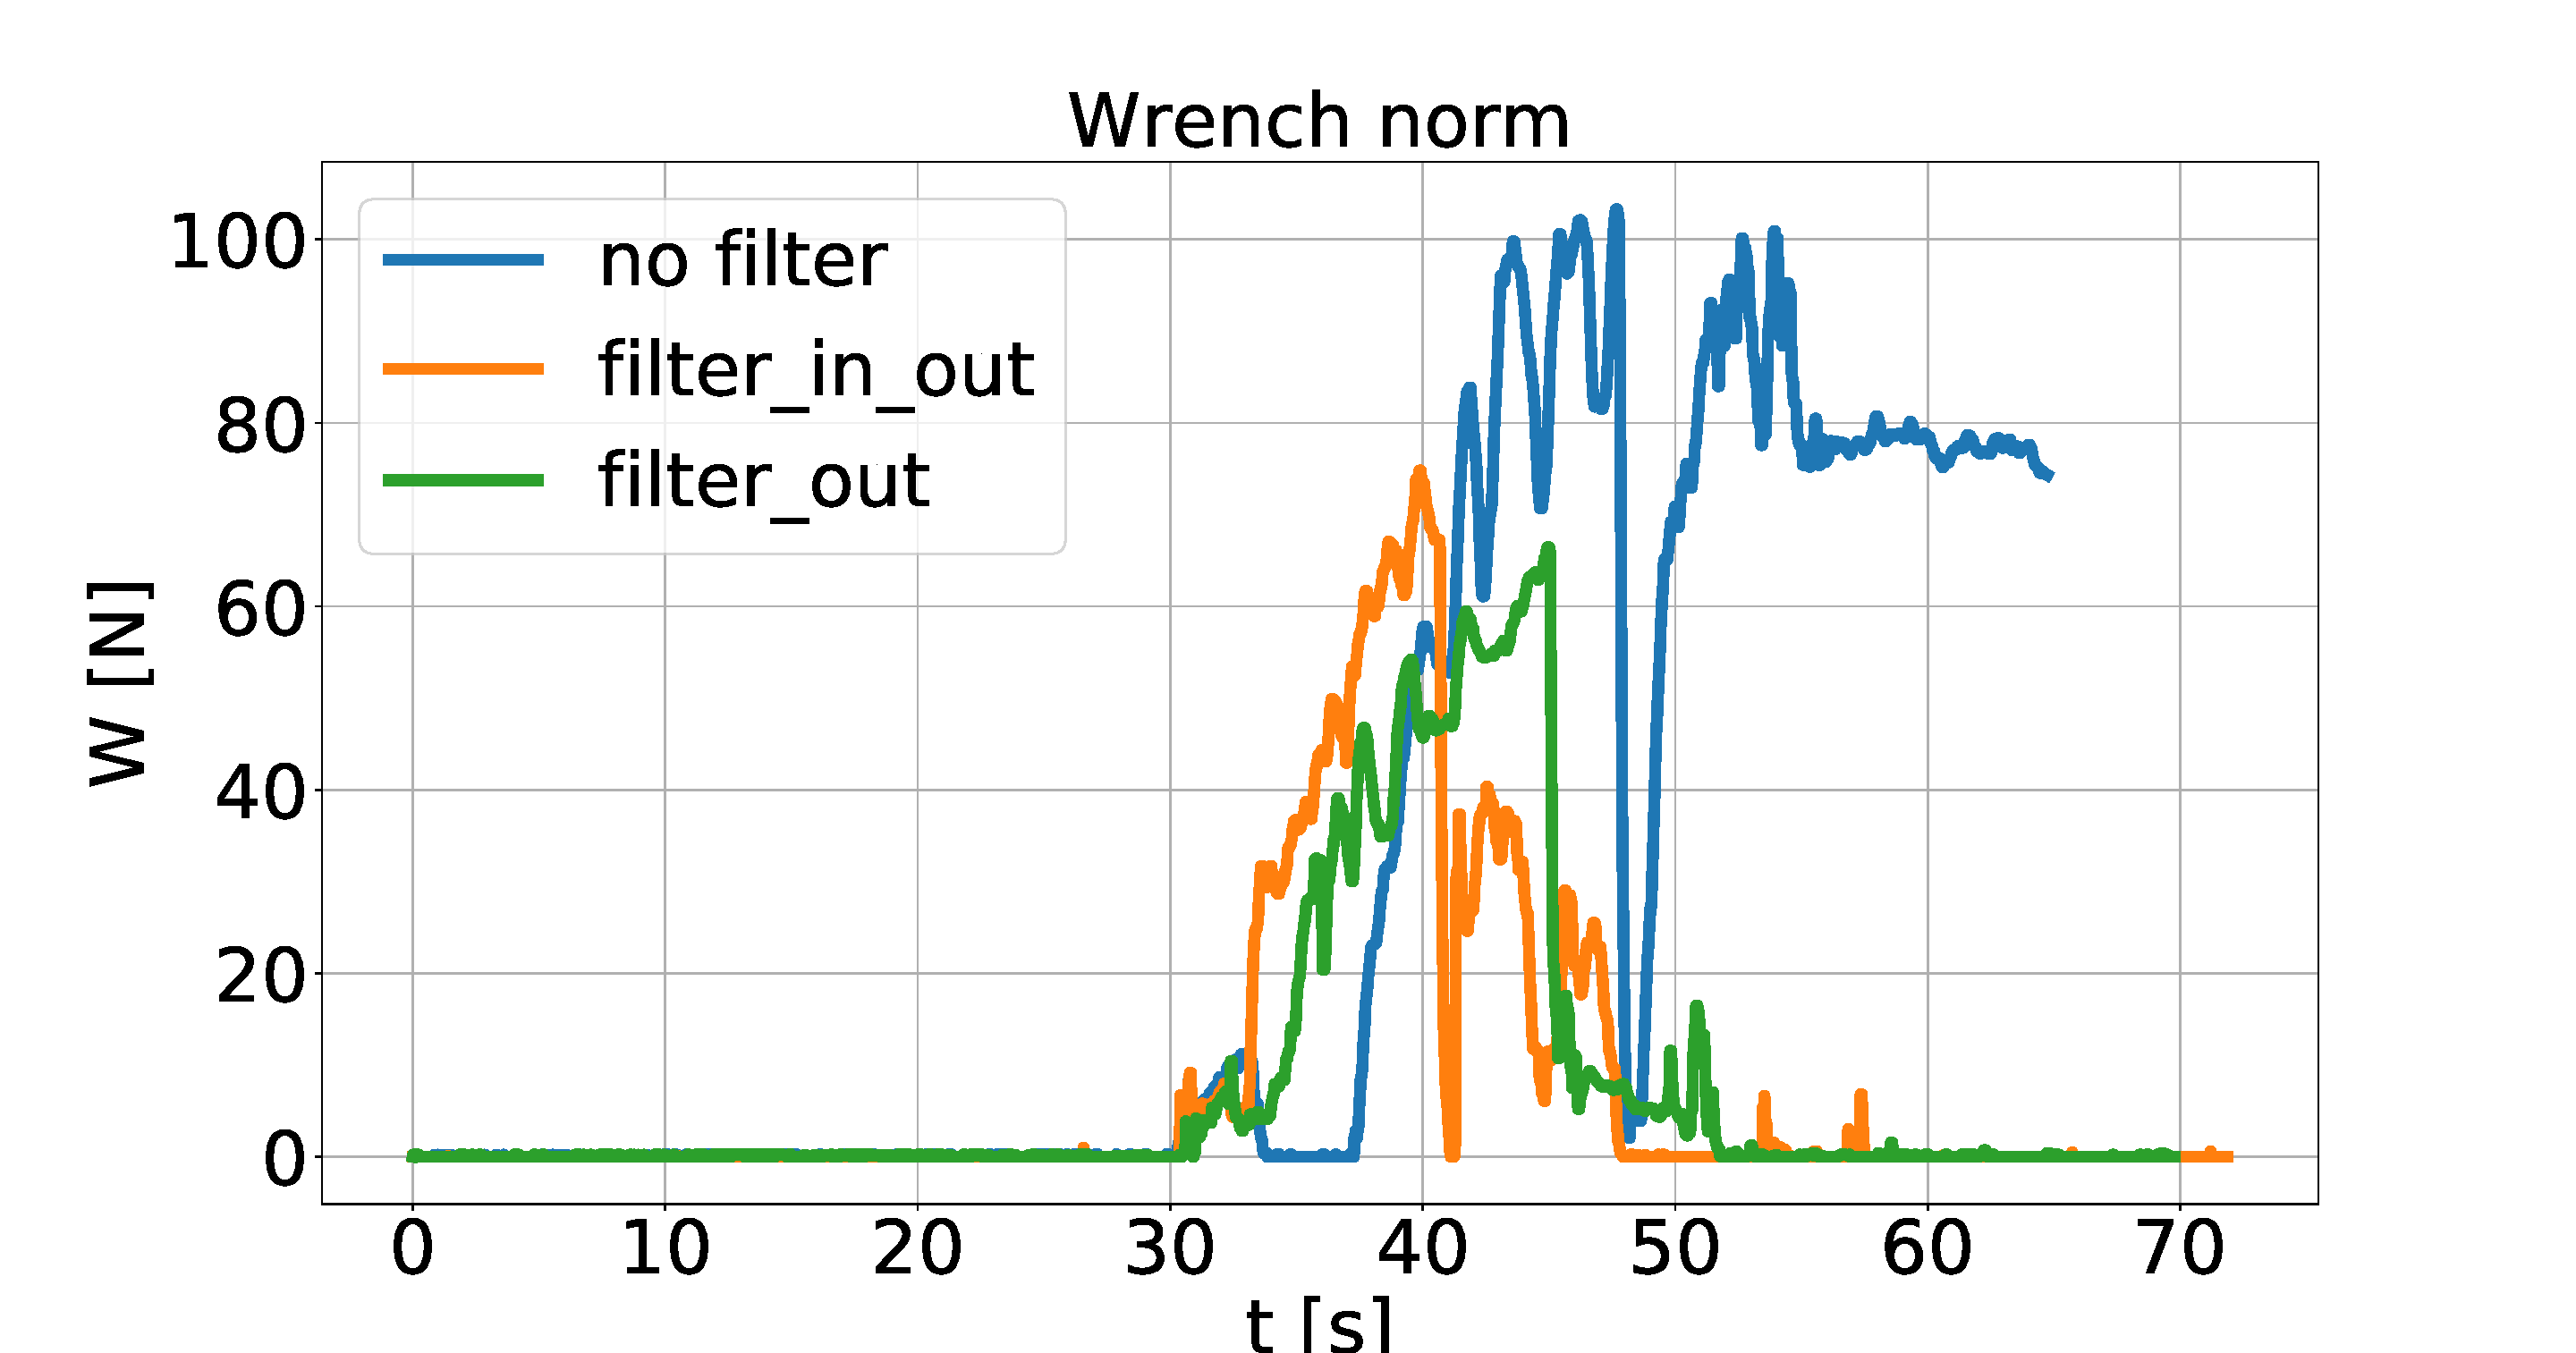
\includegraphics[width=\linewidth]{figures/hardware_experiments/wrench_norm.pdf}
    \caption{Caption here Average wrench 68 vs 34 N}
\end{subfigure}
\hspace*{-0.2cm} 
\begin{subfigure}{0.9\columnwidth}
    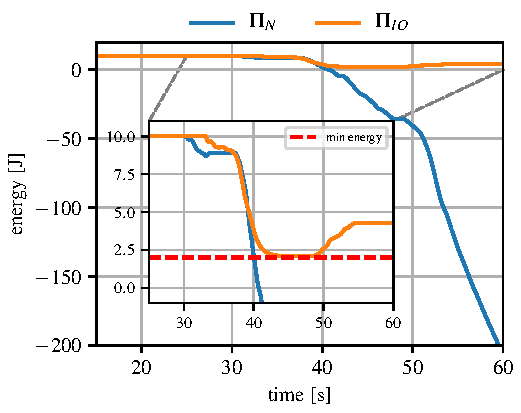
\includegraphics[width=\linewidth]{figures/hardware_experiments/energy_tank.pdf}
    \caption{Caption here.}
\end{subfigure}
    \caption{Caption}
    \label{fig:passivity_experiment}
\end{figure}

The goal of the hardware experiment is to demonstrate that the algorithm can be deployed on a real platform at high control rates. For this purpose, we perform a door opening experiment similarly to the description provided in the previous section. The door motion and the robot base are tracked via a VICON system, eliminating the need for precise state estimation. We plan to remove this limitation in future work. The door motion is limited using a rope which is cut counting 3 seconds after the energy in the tank has reached the allowed minimum. We repeat the experiment for methods $\Pi_{N}$ and $\Pi_{IO}$ recalling that the last controller only uses the passivity constraint in the outer loop. The wrench norm and the evolution of the energy in the tank during the experiments can be seen in \fig \ref{fig:passivity_experiment}. As one can see in the accompanying video, without passivity, the manipulator exert a rapidly increasing wrench up to the point of breaking the rope apart. On the other hand, when passivity is ensured, the power flow and external wrench is regulated leading to a robust interaction behavior and no need for the operator intervention. When the object is released, the gripper gets stuck in a constrained configuration between the door plate and the handle. When $\Pi_{N}$ is deployed, the controller tries to push aggressively and is therefore not able to escape this gripper trap. When using $\Pi_{IO}$ instead, the tank residual energy is low and aggressive actions are prohibited. The overall behavior is safer and allows the robot to escape from the bad configuration.  

% In order to qualitatively evaluate the algorithm's replanning capabilities, we disturb the manipulator during the opening phase, releasing the contact between the handle and the finger. As we can see in the accompanying video, the controller is able to re-plan a feasible trajectory to the handle and successfully perform the task. 

\section{Method limitations}
We conclude the validation section with a qualitative discussion on the method limitations which can highlight future work directions. In the following we describe to which elements one need to take particular care and could be extended to improve the propose method.

\subsection{Model mismatch}
Problem with poor geometric knowledge

\subsection{Cost tuning}
Mention the frame positioning and the cost deadband

\subsection{Sim to Real Gap}
